%
% frames.tex
%
% (c) 2019 Prof Dr Andreas Müller, Hochschule Rapperswil
%
\section{Frames
\label{section:frames}}
\rhead{Frames}
Eine orthonormierte Basis eines Hilbertraumes ist sehr starr.
Es ist nicht möglich, auch nur einen einzigen Vektor ein kleines
Bisschen zu ändern, ohne die Eigenschaften, die zum Satz~\ref{satz:parseval}
geführt haben, zu zerstören.
Im Hinblick auf die numerische Behandlung von Signalen ist das
ein unerwünschter Zustand.
Rundungsfehler werden unvermeidlich dazu führen, dass solche strengen
Strukturen nur näherungsweise im Computer nachgebildet werden 
können.

Die Zerlegung eines Vektors $v$ in einer Orthonormalbasis enthält keine
Redundanz.
Geht einer der Koeffizienten $\hat{v}_k$ verloren, gibt es keine
Chance, den Vektor zu rekonstruieren.
Auch diese Situation ist unerwünscht, denn durch Rundungsfehler geht
mindestens ein Teil der Information in einem Koeffizienten verloren.
Wir suchen daher nach einer Verallgemeinerung des Basis-Begriffs, welche
auf kontrollierte Weise Redundanz in die Koeffizienten $\hat{v}_k$
bringt und damit eine robustere Konstruktion ermöglicht.

\subsection{Ein geometrisches Beispiel
\label{subsection:hexagon}}
\begin{figure}
\centering
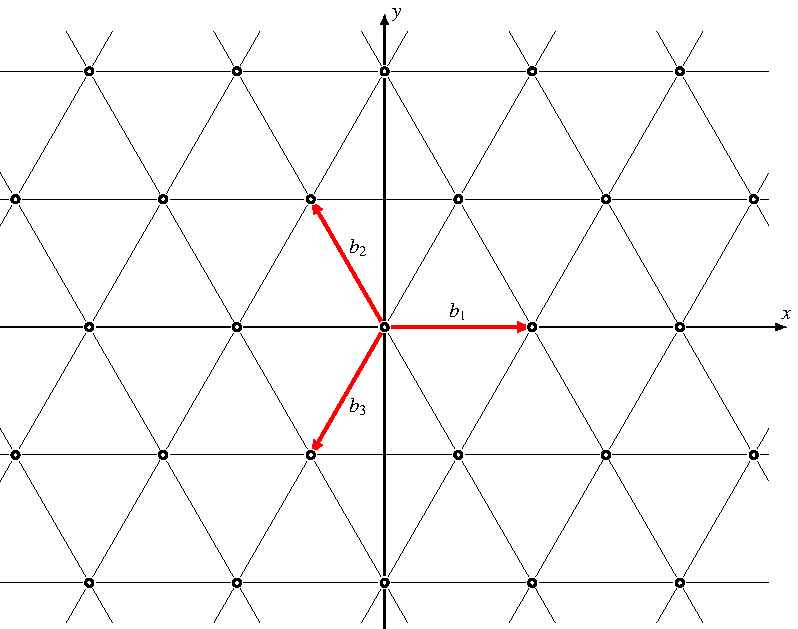
\includegraphics{chapters/1-geometrie/images/hexagon.pdf}
\caption{Sechseck-Gitter in der Ebene zum Frame $\{b_1,b_2,b_3\}$.
\label{geometrie:hexagon:image}}
\end{figure}
Wir suchen ein geeignetes Koordinatensystem, um ein Problem über
Bienenwaben in der Ebene zu lösen.
Dazu gehört das hexagonale Gitter in Abbildung~\ref{geometrie:hexagon:image}.
Selbstverständlich kann dafür das übliche rechtwinklige Koordinatensystem
verwendet werden, aber die Ecken eines Sechsecks shaben darin die nicht
sehr symmetrischen Koordinaten
\begin{center}
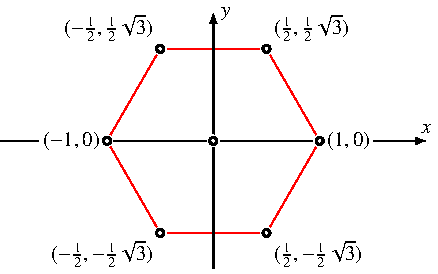
\includegraphics{chapters/1-geometrie/images/hexagon1.pdf}
\end{center}
(Siehe auch Abbildung~\ref{geometrie:hexagon:image}).
Eine bessere Variante ist das Koordinatensystem auf der Basis der beiden
Basisvektoren (in kartesischen Koordinaten)
\[
b_1 = \begin{pmatrix} 1\\0\end{pmatrix}
\qquad
\text{und}
\qquad
b_2 = \begin{pmatrix} -\frac12\\\frac12\sqrt{3}\end{pmatrix}.
\]
In diesem Koordinatensystem haben die Ecken des Sechsecks die Koordinaten
\begin{center}
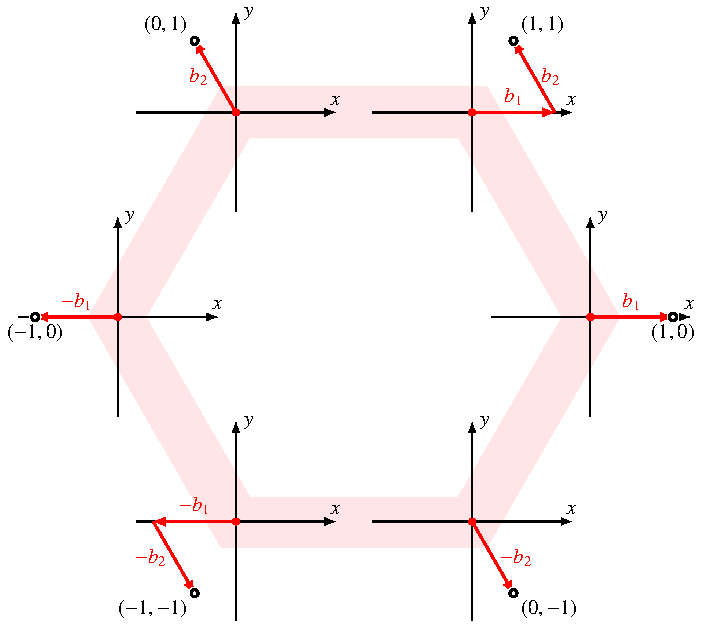
\includegraphics{chapters/1-geometrie/images/hexagon2.pdf}
\end{center}
%\begin{center}
%\begin{tikzpicture}
%\def\a{1.8}
%\foreach \p in {0,60,...,360}{
%	\draw[line width=0.1pt] ({\a*cos(\p)},{\a*sin(\p)})--
%		({\a*cos(\p+60)},{\a*sin(\p+60)});
%}
%\foreach \p in {0,60,...,300}{
%	\fill[color=white] ({\a*cos(\p)-0.65},{\a*sin(\p)-0.25})
%		rectangle ({\a*cos(\p)+0.65},{\a*sin(\p)+0.25});
%}
%
%\node at (0,0) {$0$};
%\node at ({\a},0) {$(1,0)$};
%\node at ({-\a},0) {$(-1,0)$};
%\node at ({0.5*\a},{\a*sqrt(3)/2}) {$(1,1)$};
%\node at ({0.5*\a},{-\a*sqrt(3)/2}) {$(0,-1)$};
%\node at ({-0.5*\a},{\a*sqrt(3)/2}) {$(0,1)$};
%\node at ({-0.5*\a},{-\a*sqrt(3)/2}) {$(-1,-1)$};
%\end{tikzpicture}
%\end{center}
%\begin{align*}
%&      &&(0,1)  &&(1,1)&&     \\
%&(-1,0)&&       &&      &&(1,0)\\
%&      &&(-1,-1)&&(0,-1)&&
%\end{align*}
Was bereits viel besser aussieht.
Trotzdem ist auch dies noch nicht ganz zufriedenstellend. 
Zum Beispiel sind die Ecken links oben und rechts unten direkt durch den
Basisvektor $b_2$ darstellbar, die Ecken rechts oben und links unten
dagegen nur durch eine Linearkombination.
Wir könnten natürlich auch die linke untere Ecke als Basisvektor nehmen,
dann würde eiinfach die linke obere Ecke speziell.
In dieser Situation lässt es sich also mit einer Basis gar nicht erreichen,
dass alle Eckpunkte sich auf einfache Art darstellen lassen.

Verzichten wir jedoch daruf, dass die Vektoren linear unabhängig sein müssen,
können wir also ``Basis'' die drei Vektoren (in kartesischen Koordinaten)
\begin{align}
b_1
&=
\begin{pmatrix}1\\0\end{pmatrix}
&
b_2
&=
\begin{pmatrix}-\frac12\\\frac12\sqrt{3}\end{pmatrix}
&
b_3
&=
\begin{pmatrix}-\frac12\\-\frac12\sqrt{3}\end{pmatrix}
\label{hexagonbasis}
\end{align}
verwenden.
Die drei Vektoren haben alle die Länge $1$, aber sie sind nicht
orthogonal, sondern haben das Skalarprodukt
\[
\langle b_j,b_k\rangle
=
\begin{cases}
-\frac12&\qquad j\ne k\\
1&\qquad j=k.
\end{cases}
\]
Zu jedem Vektor $v\in\mathbb R^2$ können wir wieder eie Koeffizienten
$\hat{v}_k=\langle v,b_k\rangle$ berechnen und damit die Linearkombination
\[
v' = \sum_{k=1}^3 \hat{v}_k\,b_k
\]
bilden,
doch es ist $v\ne v'$.
Wir berechnen die Synthese für die Basisvektoren:
\begin{align*}
b_1'
&=
b_1 - \frac12 b_2 - \frac 12 b_3
=
\frac32b_1
\\
b_2'
&=
-\frac12 b_1 + b_2 -\frac12 b_3
=
\frac32b_2
\\
b_3'
&=
-\frac12b_1-\frac12 b_2 + b_3
=
\frac32b_3
\end{align*}
Die Synthese liefert also nicht den ursprünglichen Vektor, sondern
\begin{equation}
\sum_{k=1}^3 \hat{v}_k b_k = \frac32\,v
\label{geometrie:32beispiel}
\end{equation}
zurück, das $\frac32$-fache davon.
Dies ist bereits ein Ausdruck der Tatsache, dass die Information in den
Koeffizienten $\hat{v}_k$ redundant ist.
Andererseits zeigt dies auch, dass alle Richtungen gleichermassen
verzerrt werden.

Diese Vektoren sind natürlich nicht mehr linear unabhängig, Vektoren
der Ebene können also auf verschieden Art linear aus den $b_k$ kombiniert
werden.
Da $b_1+b_2+b_3=0$ ist, kann man zu den Koeffizienten $\hat{v}_k$
eine beliebige Zahl $\alpha$ hinzuaddieren, und erhält
\[
\sum_{k=1}^3 (\hat{v}_k+\alpha)\, b_k
=
\sum_{k=1}^3 \hat{v}_k\,b_k
+\alpha
\sum_{k=1}^3 b_k
=
\sum_{k=1}^3 \hat{v}_k\,b_k
=
\frac32 v.
\]
Die modifizierten Koeffizienten ergeben also das gleichen synthetisierten
Vektor $\frac32 v$.

Für die Norm des synthetisierten Vektors gilt natürlich
\[
\|v'\|^2
=
\frac94\|v\|^2
=
\sum_{k=1}^3 \hat{v}_k^2 
-
\frac12\sum_{k\ne l} \hat{v}_k\hat{v}_l.
\]
%Die modifizierten Koeffizienten ergeben natürlich dieselbe Norm, also
%\begin{align*}
%\|v'\|^2
%&=
%\sum_{k=1}^3 (\hat{v}_k+\alpha)^2 
%-
%\frac12\sum_{k\ne l} (\hat{v}_k+\alpha)(\hat{v}_l+\alpha).
%\\
%&=
%\sum_{k=1}^3 \hat{v}_k^2
%+2\alpha \sum_{k=1}^3 \hat{v}_k
%+3\alpha^2
%-
%\frac12\sum_{k\ne l} \hat{v}_k\hat{v}_l
%-
%\sum_{k\ne l} \hat{v}_k \alpha
%-
%3\alpha^2
%\end{align*}


Was zeichnet die Koeffizienten $\hat{v}_k$ gegenüber den modifizierten
Koeffiziente $\hat{v}_k$ aus?
In Abbildung~\ref{3dbasisbild} sind die Koeffizienten $\hat{v}_k$ als
dreidimensionaler Vektor $v'$ dargestellt.
Punkte in der Ebene werden durch die Analyse mit Hilfe der Vektoren $b_k$
auf Vektoren in der hellblau hervorgehobenen Ebene abgebildet.
Die alternativen Linearkombinationen entstehen, indem man zu $v$
ein Vielfaches des grünen Normalenvektors $n$ hinzuaddiert.
Die gelb gezeichneten Punkte $w$ bilden eine Gerade senkrecht
auf der hellblauen Ebene.
Alle Punkte auf dieser Geraden führen auf die gleiche
Linearkombination $\frac32v$.
Die mit Hilfe der Skalarprodukte gefundene Linearkombination
$\hat{v}_k=\langle v,b_k\rangle$ hat daher die Eigenschaft, 
$v'$ unter all den Punkte auf der Geraden die kürzeste Länge hat.
Oder: die Koeffizienten $\hat{v}_k$ zeichnen sich unter allen
Koeffizienten $v_k$ mit der gleichen Linearkombination dadurch aus, 
dass
\begin{equation}
\|v'\|^2
=
\sum_{k=1}^n |\hat{v}_k|^2
\le
\sum_{k=1}^n |v_k|^2
\qquad
\text{für Koeffizienten $v_k$ mit}
\quad
\sum_{k=1}^3 \hat{v}_kb_k
=
\sum_{k=1}^3 v_kb_k
\label{hexagonbasiseigenschaft}
\end{equation}
ist.
Die durch $\hat{v}_k$ gefundenen Koeffizienten zeichnen sich durch
die minimale ``Koeffizientenenergie'' aus.

Im Falle einer Orthonormalbasis konnte man dank der Plancherel-Formel
die Norm eines Vektors mit Hilfe der Quadratsumme der Koeffizienten
berechnen.
Die Eigenschaft \eqref{hexagonbasiseigenschaft} kann also als erweiterte
Form der Plancherel-Formel angesehen werden.

\begin{figure}
\centering
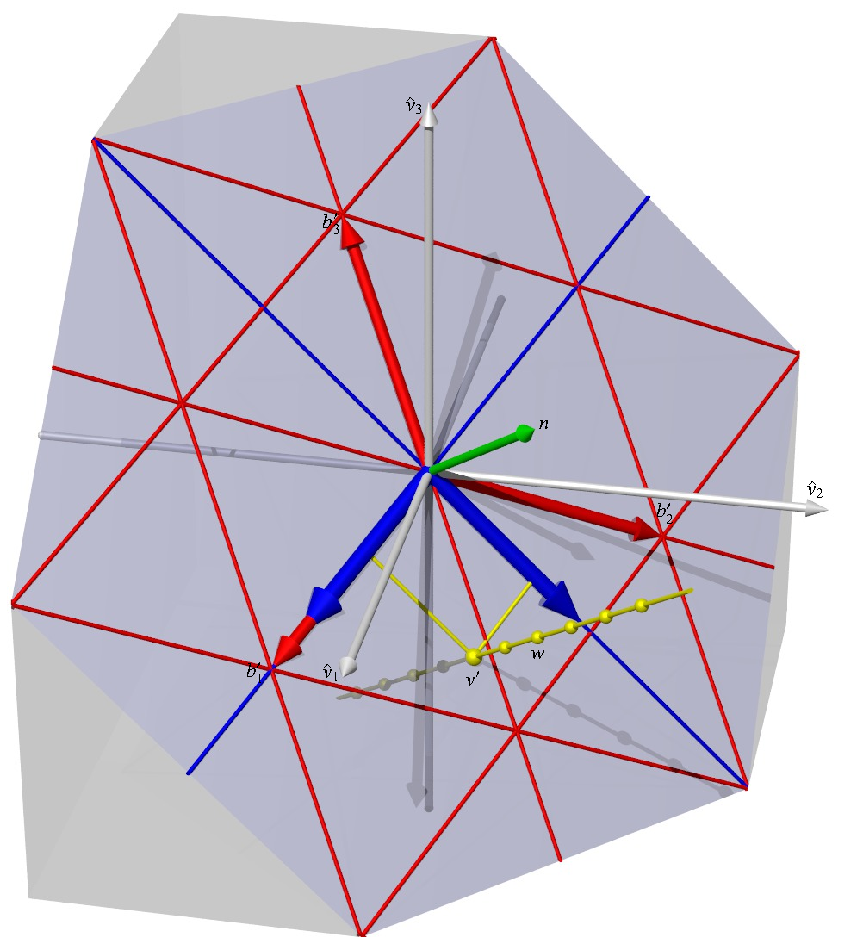
\includegraphics{chapters/1-geometrie/images/tri.pdf}
\caption{Darstellung der Koeffizienten $\hat{v}_k$ bezüglich Vektoren $b_i$
aus \eqref{hexagonbasis}.
Die drei Vektoren $b_i$ haben als $\hat{v}_k$-Koeffizienten-Vektoren
die Vektoren $b_i'$.
Die $x$- und $y$-Achsrichtung werden auf die beiden blauen Vektoren
abgebildet.
Ein Vektor $v$ wird auf den Vektor $v'$ mit den Komponenten
$\hat{v}_k$ abgebildet.
Die Darstellung eines Vektors als Linearkombination der $b_i$ ist
jedoch nicht eindeutig.
Ändert man die Koeffizienten um den gleichen Wert, was gleichbedeutend damit
ist, dass man dem Vektor $v'$ ein Vielfaches von $n$ hinzufügt, entsteht
bei der Synthese $\sum \hat{v}_k b_k$ der gleiche Punkt.
Alle gelben Punkte $w$ sind daher Koeffizienten, die den gleichen Punkt $v$
ergeben, wenn man damit die Vektoren $b_i$ linear kombiniert.
\label{3dbasisbild}}
\end{figure}

\subsection{Definition eines Frames}
Nach dem motivierenden Beispiel im vorangegangenen Abschnitt sind wir nun
bereit, eine allgemeine Definition aufzubauen.
Wir wollen also weiterhin die Vektoren eines Vektorraums $V$ mit Hilfe
einer Menge von Vektoren $\{e_k\,|\,1\le k\le n\}$ linear kombinieren,
verlangen aber nicht mehr, dass die Vektoren $e_k$ linear unabhängig sind.
Dies bedeutet natürlich, dass die Darstellung eines Vektors $v\in V$
nicht mehr eindeutig sein wird.

Nicht jede Menge von Vektoren $\{e_k\,|\,1\le k\le n\}$ ist geeignet.
Es muss ja immer noch jeder Vektor dargestellt werden können, das
Erzeugnis der Vektoren muss also der ganze Vektorraum sein:
\[
U
:=
\langle e_k\,|\,1\le k\le n\rangle
=
V.
\]
Wäre das Erzeugnis nur ein echter Unterraum $U\subset V$, dann gäbe es
einen Vektor $b\in V$, der senkrecht steht auf allen $b\perp V$.
Wir fordern daher, dass es keinen Vektor gibt, der auf allen Vektoren $e_k$
senkrecht steht.

Damit die Berechnung effizient bleibt, möchten wir weiterhin nur mit den
Koeffizienten $\hat{v}_k = \langle v,e_k\rangle$ arbeiten müssen.
Für eine Orthonormalbasis hat die Plancherel-Formel gezeigt, dass
\[
\sum_{k=1}^n |\hat{v}_k|^2 = \| v \|.
\]
In der aktuellen Situation können wir nicht mehr erwarten, dass dies 
weiterhin funktioniert.
Wir müssen aber mindestens verlangen, dass die Transformation
\[
\mathcal{T}
\colon
V\to \mathbb R^n
:
v\mapsto \hat{v}_k
\]
stetig ist, dass sich also kleine Änderungen von $v$ ebenfalls
kleinen Änderungen des Vektors der $\hat{v}_k$ auswirken.
Es muss also eine Konstante $B$ geben, so dass
\[
\sum_{k=1}^n |\hat{v}_k|^2
=
\sum_{k=1}^n |\langle v,e_k\rangle|^2
\ge
A \| v \|^2.
\]

Wir müssen aber auch sicherstellen, dass die Rekonstruktion des Vektors $v$
auf stetige Art von den Koeffizienten $\hat{v}_k$ abhängt. 
Eine kleine Änderung der Koeffizienten darf sich nur in beschränkten Änderungen
im rekonstruierten Vektor $v$ auswirken.
Es muss also eine Konstante $B$ geben, so dass
\[
\sum_{k=1}^n |\hat{v}_k|^2
=
\sum_{k=1}^n |\langle v,e_k\rangle|^2
\le
B \| v \|^2
\]
gilt.

Damit haben wir alle Elemente zusammen für die folgende Definition,
die auch für unendlichdimensionale Hilberträume funktioniert.

\begin{definition}
\label{definition:frame}
Eine Teilmenge $\{ e_k\,|\, k\in K\}\subset V$ heisst ein {\em Frame},
wenn es zwei von $0$ verschiedene Konstanten $A$ und $B$ gibt, so dass
\[
A\|v\|^2 \le \sum_{k\in K} |\langle v, e_k\rangle|^2 \le B \| v\|^2
\]
gilt für jeden Vektor $v\in V$.
Die Konstanten $A$ und $B$ heissen die {\em Framekonstanten} des Frames.
Das Frame heisst {\em straff}, wenn $A=B$ ist.
\end{definition}

\begin{beispiel}
Das Beispiel von Abschnitt~\ref{subsection:hexagon} ist ein Frame.
Die Formel \eqref{geometrie:32beispiel} zeigt, dass die Framekonstanten
des Frames $A=B=\frac32$ ist.
Das Frame ist also sogar straff.
\end{beispiel}

In der Definition wird nicht erwähnt, dass die Vektoren des Frames den
ganzen Raum aufspannen müssen.
Diese Eigenschaft folgt jedoch direkt aus der Definition eines Frames,
wie der folgende Satz zeigt.

\begin{satz}
Ist $\mathcal{B}=\{ e_k\,|\, k\in K\}$ ein Frame des Hilbertraumes $V$
mit Framekonstanten $A$ und $B$, dann gibt es keinen Vektor $v\in V$,
der auf allen Vektoren $e_k$ senkrecht steht.
\end{satz}

\begin{proof}[Beweis]
Nehmen wir an, es gäbe einen Vektor $v\in V$ mit $\langle v,e_k\rangle=0$
für alle $k\in K$.
Dann folgt aus den Frame-Ungleichungen
\[
\| v \|^2 \le \frac1{A} \sum_{k\in K} |\langle v,e_k\rangle|^2 = 0
\qquad\Rightarrow\qquad
v=0.
\]
Der Nullvektor ist also der einzige Vektor, der auf allen Framevektoren
senkrecht steht.
\end{proof}

Eine orthonormierte Basis war die bevorzugte Wahl für eine Basis, weil
sich damit die Transformation $\mathcal{T}$ besonders leicht invertieren
lässt.
Der Satz~\ref{satz:parseval} hat gezeigt, dass die Transformation %$\mathcal{T}$
eine Isometrie ist, insbesondere gilt
\[
\|v\|^2
=
\sum_{k\in K} |\hat{v}_k|^2
=
\sum_{k\in K} |\langle v,e_k\rangle|^2.
\]
Dies bedeutet, dass eine orthonormierte Basis ein straffes Frame mit
Framekonstanten $A=B=1$ ist.
Umgekehrt drängt sich die Frage auf, ob straffe Frames oder spezielle
Werte der Frame-Konstanten eine besondere Bedeutung für die Invertierbarkeit
haben.

\begin{figure}
\centering
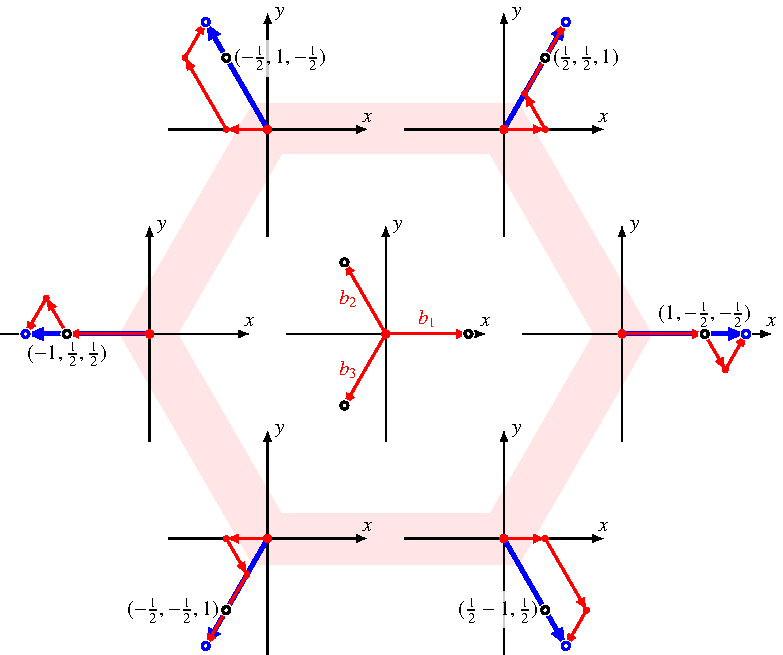
\includegraphics{chapters/1-geometrie/images/hexagon3.pdf}
\caption{Rekonstruktion bei einem straffen Frame.
Das Frame bestehend aus den Vektoren $\{b_1,b_2,b_3\}$ ist straff
mit der Framekonstanten $A=\frac32$.
Die mit den Skalarprodukten gewichtete Linearkombination der
Framevektoren liefert nicht den ursprünglichen Vektor zurück, sondern
einen Vektor, der mit der Framekonstanten multipliziert wird.
Gezeigt wird dies für die sechs Ecken des Hexagons.
Die Skalarprodukte mit den Framevektoren, die Framekoordinaten, sind
als Zahlentripel bei jedem Punkt angegeben.
Die roten Vektorpfade stellen die Linearkombination dar, die blauen
Vektoren die Summe.
\label{geometrie:hexagon:rekonstruktion}}
\end{figure}

\subsection{Allgemeine Frames}
Die Wahl der Indexmenge $K$ in der Definition~\ref{definition:frame}
war einigermassen willkürlich.
Schon bei der Fouriertransformation ist eine solche diskrete Menge
für die Indizierung der Vergleichsfunktionen nicht mehr ausreichend.
Dort werden nämlich die Funktion $e^{i\omega t}$ mit $\omega\in\mathbb R$
verwendet.
Auch die geplante Anwendung auf Wavelets ist davon betroffen.
Dort wollen wir mit Funktionen $\psi_{a,b}$ vergleichen, die 
skalierte und verschobene Versionen eines Mutter-Wavelets $\psi$ sind,
mit Skalierungsfaktor $a\in\mathbb R^*$ und $b\in \mathbb R$.

Lässt man eine beliebige Indexmenge zu, ist die Definition der
Transformation $T$
\[
k
\mapsto
(Tv)(k) = \langle v,e_k\rangle
\]
als komplexwertige Funktion auf $K$ immer noch sinnvoll.
Für eine überabzählbare Indexmenge $K$ ist die Summe 
\[
\sum_{k\in K} |\langle v,e_k\rangle|^2,
\]
die in der Definition eines Frames auftritt, schlicht sinnlos.
Wir stehen hier also vor einem ähnlichen Problem wie bei der Frage,
wie man aus dem Raum der Signale auf $\mathbb R$ einen Hilbertraum machen kann.
Diese Frage wird in Kapitel~\ref{chapter:fourier} im Detail beantwortet.

Nehmen wir für den Moment an, dass es gelungen ist, eine Hilbertraum $H$
von Funktionen auf $K$ zu konstruieren.
Die Frame-Ungleichung kann dann mit Hilfe der Norm von $H$ formuliert
werden, sie lautet
\[
A\|v\|^2 \le \|Tv\|^2 \le B\|v\|^2.
\]
Die Norm in der Mitte ist als Norm in $H$ zu lesen.
Diese Ungleichungen sagen immer noch aus, dass kein Vektor $v\in V$ bei
der Transformation $T$ ``unsichtbar'' wird.
Wäre nämlich $Tv=0$ in $H$, dann wäre auch $\|Tv\|=0$ und damit
$\|v\|=0$.
Die Frame-Ungleichung stellt also sicher, dass die Abbildung $T$ 
injektiv und damit potentiell invertierbar ist.

Es ist aber keinesfalls garantiert, dass das Bild der Transformation $T$
den ganzen Hilbertraum $T$ abdeckt, ganz im Gegenteil.
Schon im Beispiel in Abschnitt~\ref{subsection:hexagon} wurde gezeigt,
dass die mit Hilfe eines Frames gefundenen Koeffizienten redundant sind.
Alle Vektoren der Menge
\[
\left\{
\left.
\begin{pmatrix}\hat{v}_1\\\hat{v}_2\\\hat{v}_3\end{pmatrix}
+\alpha\begin{pmatrix}1\\1\\1\end{pmatrix}
\,
\right|\,
\alpha \in\mathbb R
\right\}
\]
beschreiben den gleichen Punkt in der Ebene, aber nur einer davon 
wird von der Transformation $T$ erreicht.
Dies entspricht natürlich genau dem, was man erwartet: der Bildraum
der Ebene $\mathbb R^2$ unter der Abbildung $T$ ist ein zweidimensionaler
Teilraum des $\mathbb R^3$.

Die Abbildung $T$ wird daher im Allgemeinen nicht invertierbar sein, aber
wir dürfen hoffen, dass es eine Formel gibt, mit der man aus $Tv$ den 
Vektor $v$ rekonstruieren kann.
Im Falle des Beispiels war dies die Formel
\[
v = \frac23 \sum_{k=1}^3 \langle v,e_k\rangle \, e_k.
\]
Für ein beliebiges Frame ist so eine Formel natürlich wieder wegen
der Summe nicht sinnvoll.
Dach in Kapitel~\ref{chapter:fourier} werden wir sehen, dass sie sich
oft durch eine Integralformel ersetzen lässt.
Die Konstruktion eines solchen vektorwertigen Integrals ist allerdings
etwas subtil, wird kehren zu dieser Problematik im Kapitel~\ref{chapter:cwt}
zurück.


